% Chapter 4

\chapter{Methodology} % Write in your own chapter title
\label{Chapter4}
\lhead{Chapter 4. \emph{Methodology}} % Write in your own chapter title to set the page header
In this chapter we introduce and describe the real life game dataset that we got from GameAnalytics, selection of user events and building player behavior features to construct a game metric data as input to our clustering algorithm. We implemented a incremental MapReduce k-means clustering algorithm and apply it on multiple batches of the game metric data to find average player behaviors described by a the constructed player behavioral feature vector. The algorithm is highly scalable and can easily be executed on numerous virtual computers using the Amazon Elastic MapReduce (Amazon EMR) web service. 

We test the MapReduce k-means algorithm on multiple batches of the real game data. Where each batch of game data is processed in one iteration and the output is used as the input to the next batch. Using one iteration we allow for efficient computation and given the changing nature of the data over time in each batch we don't risk falling into local optimum. This method is compared against multiple iterations on the real game data and on a larger generated example, where 3 normal distributions shift between data batches.

Different MapReduce k-means implementation were tried in the process of the thesis and different efficient computational methods were compared on a larger generated dataset, including scalability tests running on different cluster setups in the Amazon EMR.

\section{Dataset}
The dataset is from a Free-to-Play (F2P) online game that is available on Google Plus and Facebook. This real life game dataset is from one of the many games that GameAnalytics is analyzing for their customers. Because of confidentiality issues we are not allowed to mention its name but lets call it \textit{Free Battle Online} (FBO). Same is about the real names of events or features in the dataset is fictional, this unfortunately means that we also have very limited knowledge about the data, e.g. what individual events mean and the timespan. The goal of FBO is to fight battles against both non-playing-characters (NPCs) and other players. You can click on various places to travel to finish battle missions or just visit other players and initiate battles to steal their resources.

The dataset is a user telemetry data, e.g. user behavioral events, where each line represents an action performed by the user or is a direct influence from a user behavior. There are over $5.000.000$ rows in this data set, with approx. $550$ unique events generated by approx. $94.000$ players. Average events per player is $\mu = 54$ with standard deviation $\sigma = 145$, indicating that the data is spread out over a wide range of values. The measure of the spread is in Table~\ref{tab:FiveSummaryEvents} showing the five number summary; The first quartile $Q_1$ cuts off the lowest $25\%$ of the data, the second quartile gives the center of the distributions known as the $Median$, the third quartile $Q_3$ cuts of the highest $25\%$. The median is lower than the mean of the data describing a positively skewed distribution, see Figure~\ref{fig:boxplot_events} for a visualization of the distribution.

\begin{table}[h]
\centering
\begin{tabular}{| l | l | l | l | l | l |}
    \hline
    & \textit{Min} & $Q_1$ & \textit{Median} & $Q_3$ & \textit{Max} \\ \hline
    Events & 1 & 4 & 23 & 61 & 10865 \\ \hline
\end{tabular}
\caption{This table shows the five number summary about the number of events generated by each unique player in the dataset.}
\label{tab:FiveSummaryEvents}
\end{table}


\begin{figure}[here]
\centerline{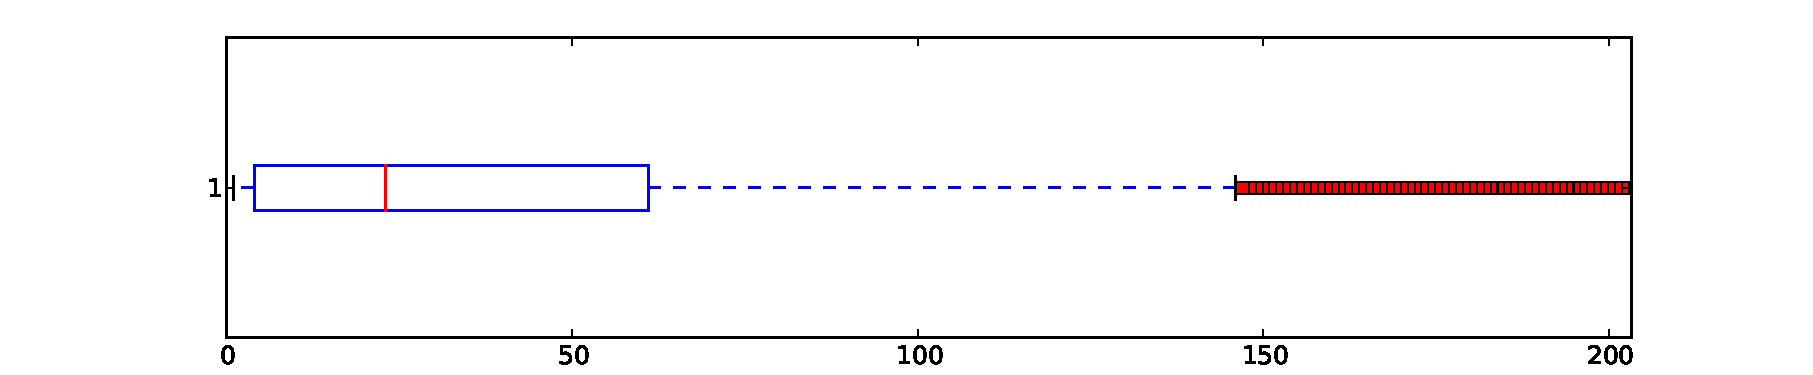
\includegraphics[width=0.9\textwidth]{Figures/boxplot_events.pdf}}
\caption{A boxplot visualizing the Events distribution incorporating the five number summary.}
\label{fig:boxplot_events}
\end{figure}

The two lines outside the box in Figure~\ref{fig:boxplot_events} are called whiskers and represent the extreme low and high values that are less than $1.5 \times IQR$ beyond the quartiles. The first and third quartiles represent the ends of the box and the median is the red line. The red \textit{squares} are individual points called \textit{outliers}. Only about $6\%$ or $\approx 5500$ players of the entire population generated more than 150 events, $0.3\%$ or $\approx300$ players have more than 1000 events and less than ten people have a range of $5.000-10.000$ generated events! A histogram showing the frequency of events generated by players is shown in Figure~\ref{fig:histogram_events_iqr}, zooming in on the spread that gives the range covered by the middle half of the data.

\begin{figure}[here]
\centerline{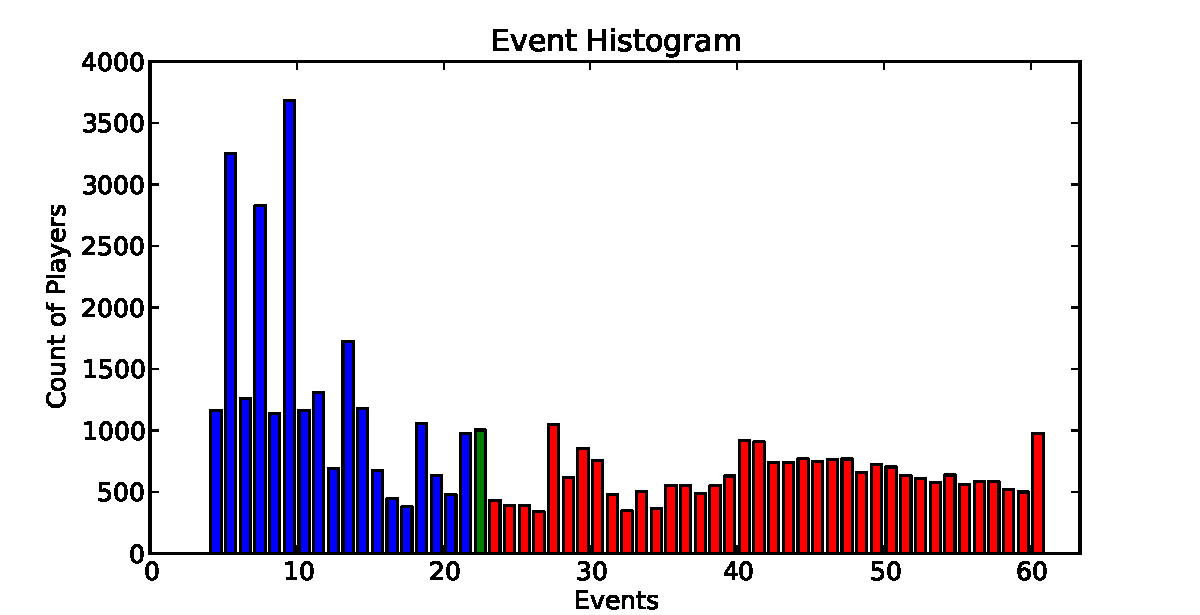
\includegraphics[width=0.9\textwidth]{Figures/histogram_events_iqr.pdf}}
\caption{A histogram for number of events using singleton buckets in the interquartile range (IQR) defined as $Q3 - Q1$, range covered by the middle half of the data.}
\label{fig:histogram_events_iqr}
\end{figure}


\subsection{Game Metric Construction}
For this thesis we tried to keep the number of game features in minimal and decided to build our feature vector with three features. Given the limited knowledge and information that we have about individual events we decided to select events that have high frequency compared to other events and hopefully could describe different behaviors between groups of players in those features. A $3-dimensional$ feature vector was constructed for each unique player, containing a frequency of three events generated by the player. The aggregated events are:
\begin{itemize}
\item Login: Number of logins/access into different areas in the game($\mu = 2.4, \sigma = 4.8$)
\item Battle: Number of battles this player have started ($\mu = 3.7, \sigma = 9.6$)
\item Premium Spending: Number of times this player spends a in-game money on virtual items or resources ($\mu = 1.1, \sigma = 2.7$) 
\end{itemize}

The five number summary of the skewed distribution is in Table~\ref{tab:FiveSummaryLoginsBattlesPremium}. Boxplots visualizing the distributions for these events are shown in relevant figures below, Logins in Figure~\ref{fig:boxplot_logins}, Battles in Figure~\ref{fig:boxplot_battles} and Premium spent in Figure~\ref{fig:boxplot_premium}.

\begin{center}
\begin{table}[h]
\centering
\begin{tabular}{| l | l | l | l | l | l |}
    \hline
    & \textit{Min} & $Q_1$ & \textit{Median} & $Q_3$ & \textit{Max} \\ \hline
    Logins & 0 & 1 & 1 & 2 & 220 \\ \hline
    Battles & 0 & 0 & 1 & 4 & 439 \\ \hline
    Premium spent & 0 & 0 & 0 & 1 & 100 \\ \hline
\end{tabular}
\caption{This table shows the five number summary for the Logins, Battles and Premium spent events generated by each unique player in the dataset.}
\label{tab:FiveSummaryLoginsBattlesPremium}
\end{table}

\begin{figure}[h]
\centerline{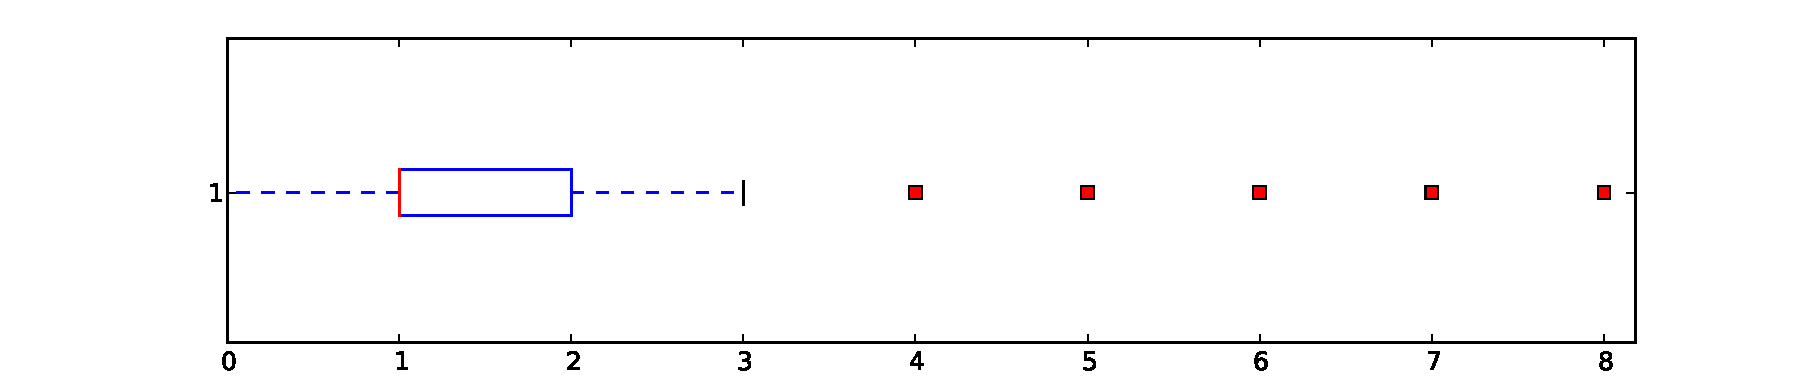
\includegraphics[width=0.9\textwidth]{Figures/boxplot_logins.pdf}}
\caption{A boxplot visualizing the Login events distribution incorporating the five number summary.}
\label{fig:boxplot_logins}
\end{figure}

\begin{figure}[h]
\centerline{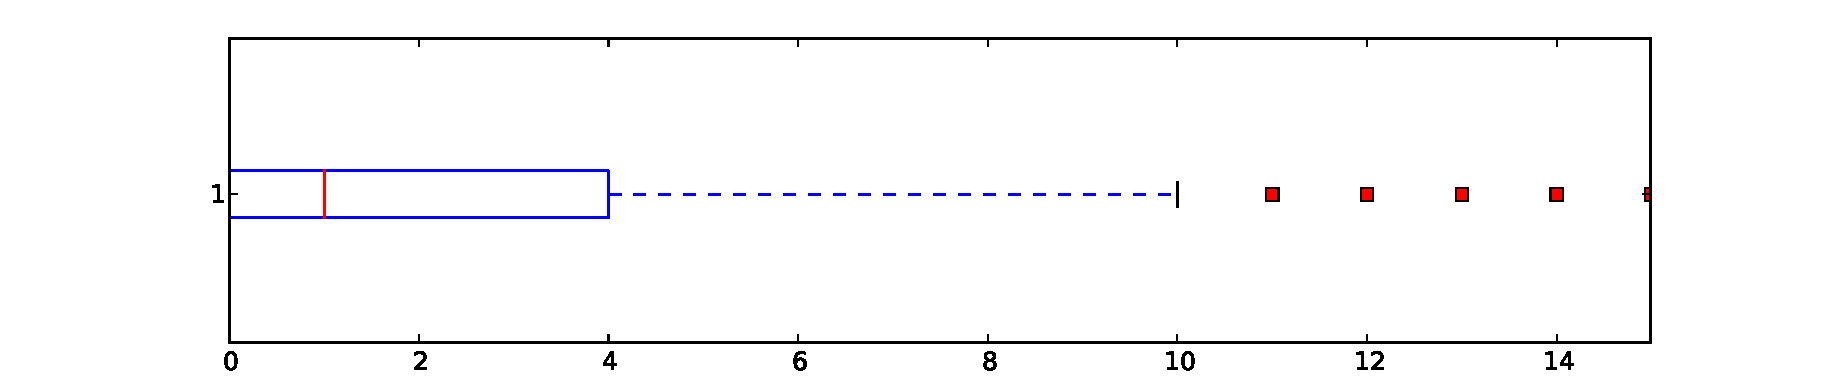
\includegraphics[width=0.9\textwidth]{Figures/boxplot_battles.pdf}}
\caption{A boxplot visualizing the Battle events distribution incorporating the five number summary.}
\label{fig:boxplot_battles}
\end{figure}

\begin{figure}[h]
\centerline{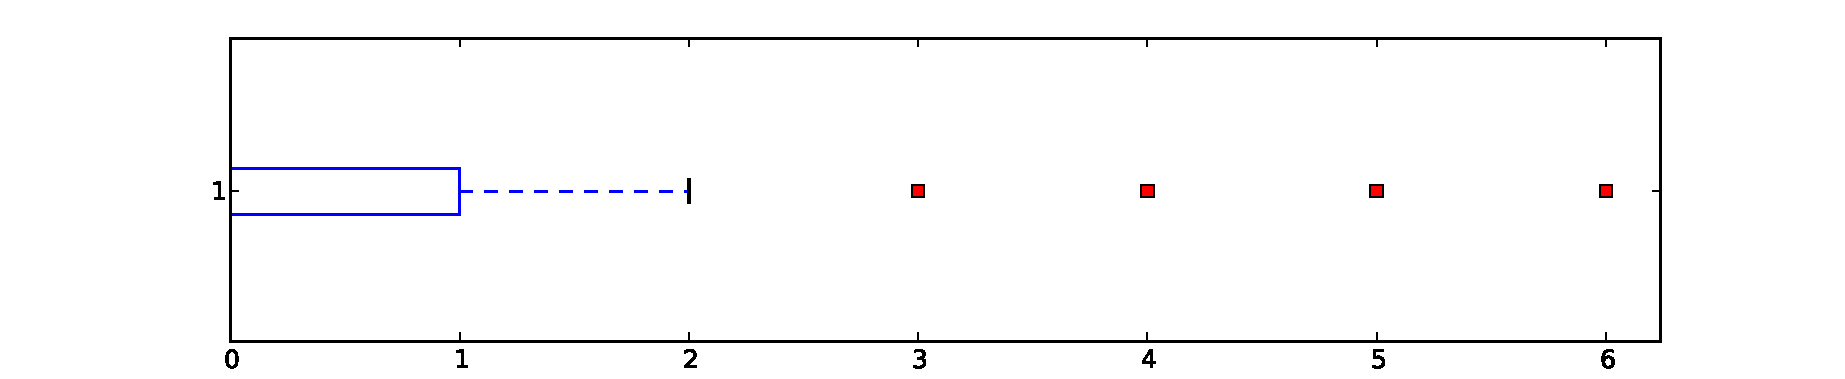
\includegraphics[width=0.9\textwidth]{Figures/boxplot_premiumspent.pdf}}
\caption{A boxplot visualizing the Premium spent events distribution incorporating the five number summary.}
\label{fig:boxplot_premium}
\end{figure}
\end{center}


\subsection{Preprocessing}
User telemetry from games can be very noisy in that sense it can contain lots of irrelevant events and logging information and even developers from the game studio can generate events. For this dataset this we performed several preprocessing steps:
\begin{itemize}
\item Sort the events after event timestamp.
\item Split the dataset into $10$ approx. equally sized pieces.
\item Filter out irrelevant events and logging information. E.g. Events not origin from Facebook or Google Plus, non related events and in game studio debugging generated events.
\item Process each piece by counting relevant events per user to build our feature vector.
\item Standardize the data using the zero mean normalization (also known as z-score), transforming it to have zero mean and unit variance insensitive to outliers.
\end{itemize}

The MapReduce k-means algorithm in this thesis takes as input multiple batches of 


\section{K-means algorithm in MapReduce}
\textit{TODO Describe the k-means algorithm implementation in MapReduce and the relevant pseudo codes and pictures}


A k-means algorithm was implemented in MapReduce that is able to process large-scale datasets. We started to implement a simple version of k-means that assigns each point to a nearest cluster in the \textit{Map} function and calculates the new centroid in the \textit{Reduce} phase. Next version had a \textit{Combiner} implemented that performs a reduce work on the same computer node as the Mapper, by calculating intermediate sums of all points for each cluster from a Map function. This minimizes the data needed to be transferred and shuffled by the MapReduce framework to the Reducer, only sending an intermediate sum with each cluster centroid from each mapper instead of list of all points in each cluster [REFERENCE]. The final k-means version uses a more efficient way of calculating the distance to the nearest centroid for each point. Using a matrix calculation that returns a distance matrix that represents distances from all points to all centroids. These different versions are compared below in respect to time and space complexity.


\subsection{K-means - Map and Reduce version}
\lipsum[1]

\subsubsection{Map}
\textit{TODO Describe the map function}

\lipsum[1-2]


\subsubsection{Reduce}
\textit{TODO Describe the Reduce function}

\lipsum[7-8]

\subsection{K-means - Map, Combine and Reduce version}
\lipsum[1]

\subsubsection{Combine}
\textit{TODO Describe the Combine function}

\lipsum[5-6]

\subsection{K-means - Efficient version}
\lipsum[1]

\subsubsection{Map}
\textit{TODO Describe the map function}

\lipsum[1-2]

\subsubsection{Combine}
\textit{TODO Describe the Combine function}

\lipsum[5-6]


\subsubsection{Reduce}
\textit{TODO Describe the Reduce function}

\lipsum[7-8]


\subsection{Distance measure}
\textit{TODO Describe the distance measure used in k-means}

\lipsum[1]


\section{MapReduce Development Environment}
\textit{TODO Describe the set-up for the experiments}
The MapReduce k-means algorithm was implemented using a framework called \textit{mrjob}~\footnote{http://pythonhosted.org/mrjob/}. Mrjob is a open-source Python framework actively maintained by Yelp~\footnote{http://opensource.yelp.com/}, that allows MapReduce jobs to be written in Python 2.5+ and executed on several platforms. Using mrjob allows for rapid implementation of MapReduce jobs by running them locally for development purposes and easily run them on your own Hadoop cluster or using the Amazon Elastic MapReduce (Amazon EMR)\footnote{http://aws.amazon.com/elasticmapreduce/}. Amazon EMR is a web service that allows developers to buy time on a Hadoop cluster to process large-scale data easily and cost-effectively.

The Python programming language was chosen for this study because GameAnalytics (GA) also uses Python and mrjob to implement their MapReduce jobs. Allowing GA easily to use and build further on the implementation from this study. 
\lipsum[1-3]